\section{Reducción del tamaño de la red de Petri en el postprocesado}
\label{sec:future-work-petri-net-reduction}

\cite{murata1989} describe en una sección titulada ``Simple Reduction Rules for Analysis''
seis operaciones que preservan las propiedades de seguridad, liveness y acotamiento de las redes de Petri.
Consulte las Definiciones \ref{definition:safeness}, \ref{definition:liveness} y \ref{definition:boundedness}
respectivamente para refrescar el significado de estas propiedades.

Las seis operaciones implican simplificaciones que reducen el número de lugares o transiciones
en la red de Petri. A continuación reproducimos los nombres utilizados para las reglas de
reducción en el documento y la Fig. \ref{fig:petri-net-reduction-rules}
representa la transformación que tiene lugar en cada caso.

\begin{enumerate}[label={\alph*)}]
  \item Fusión de lugares en serie.
  \item Fusión de transiciones en serie.
  \item Fusión de lugares paralelos.
  \item Fusión de transiciones paralelas.
  \item Eliminación de lugares de bucle.
  \item Eliminación de transiciones de bucle.
\end{enumerate}

\begin{figure}[!htb]
  \centering
  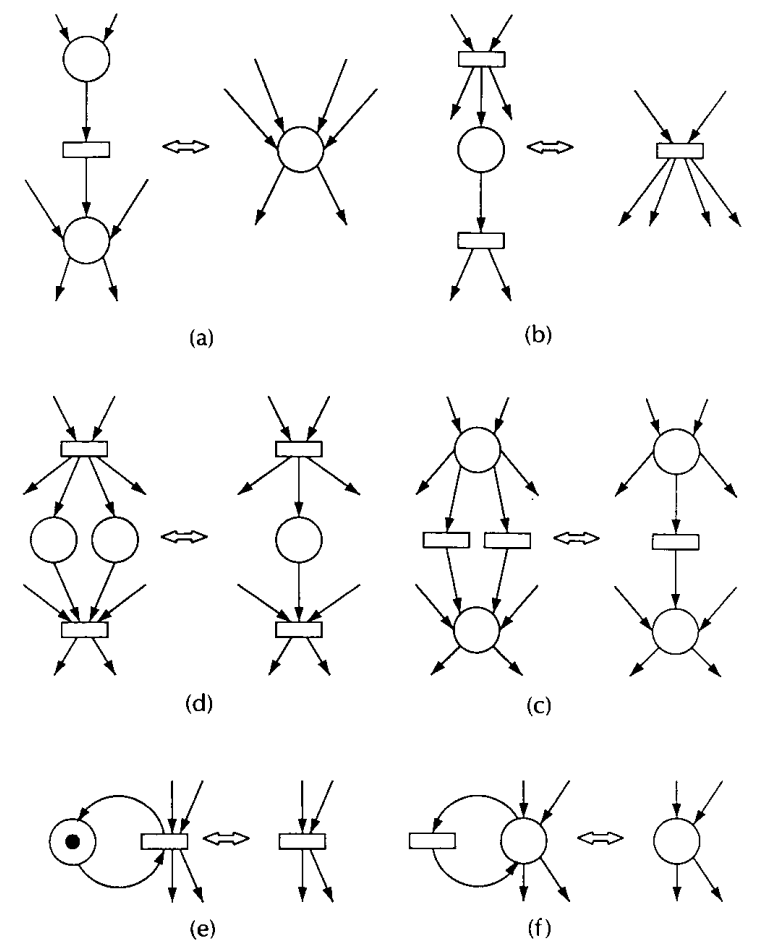
\includegraphics[width=0.9\linewidth]{petri-net-reduction-rules.png}
  \caption{Las reglas de reducción presentadas en el paper de Murata.}
  \label{fig:petri-net-reduction-rules}
\end{figure}

Como estas operaciones no afectan la propiedad de liveness, el resultado de la detección del
deadlock permanece inalterado. En consecuencia, puede resultar ventajoso reducir el tamaño de
la red de Petri tras el proceso de traducción utilizando métodos específicos disponibles en la biblioteca
\Rustinline{netcrab}. Este paso debe realizarse después de traducir todos los hilos pero antes de invocar al
verificador de modelos.

Incorporar esta funcionalidad a la propia biblioteca de redes de Petri sería más adecuado porque permitiría
que otras aplicaciones se beneficiaran de esta feature. Sería interesante investigar si este
enfoque resulta útil cuando se traducen programas más grandes que contienen cientos o miles
de lugares y transiciones.

Un inconveniente notable de la aplicación de estas operaciones es que podría ocultar el origen
del deadlock. Es valioso para el usuario disponer de información precisa sobre la línea del
código fuente donde se produce el bloqueo. Si las transiciones o lugares correspondientes que
representan esta línea se fusionan, esta información se pierde. No obstante, esta desventaja
puede considerarse aceptable cuando se trata de modelos extensos y la función podría activarse
o desactivarse a discreción del usuario.

\section{Eliminación de las rutas de limpieza de la traducción}
\label{sec:future-work-no-cleanup}

El mecanismo de gestión de errores de la \acrshort{MIR} debe tener en cuenta todos los escenarios
posibles de fallo durante el tiempo de ejecución. El objetivo del compilador \emph{rustc} es garantizar
que el código compilado falle con gracia, incluso en las circunstancias más extremas, por
ejemplo, cuando el programa se queda sin memoria o las llamadas al sistema fallan
inesperadamente debido a límites ``duros'' en los recursos disponibles u otras causas. Sin
embargo, la mayor parte de este código de limpieza de salvaguarda nunca se ejecuta en la
práctica. Los errores \acrshort{OOM} y los fallos del sistema operativo son poco frecuentes y, si llegan a
producirse, un deadlock en el código de usuario es el menor de nuestros problemas.

\cite{meyer2020} argumenta que el programa siempre terminará en un estado final de pánico una vez
que falle una sola llamada a función o aserción. En lugar de traducir el camino alternativo que sigue
la ejecución en la MIR, propone establecer un token en el lugar \Rustinline{PROGRAM_PANIC}
directamente. Esto equivale a ignorar el \acrshort{BB} de limpieza específico durante el proceso de
traducción y conectar el \acrshort{BB} al lugar \Rustinline{PROGRAM_PANIC}
como si fuera un terminador \Rustinline{Unwind} (Sec. \ref{sec:terminators}).

Esto reduce sustancialmente el tamaño del modelo de red de Petri. Tiene el inconveniente de
que se visitan \acrshort{BB} de limpieza pero nunca se conectan a otros \acrshort{BB}.
Estos deben eliminarse en un paso de postprocesamiento para no agrandar innecesariamente el modelo final.
La implementación de Meyer no parece haber realizado este paso crucial.
No está claro si la implementación se ajusta a lo
propuesto en la tesis porque el código fuente ya no puede compilarse y no hay ejemplos de
salida en el repositorio\footnote{\url{https://github.com/Skasselbard/Granite}}.

La afirmación de que el estado de pánico es irrecuperable requiere un examen exhaustivo, puesto
que hemos observado anteriormente en la introducción a Rust que el programador tiene la
opción de utilizar \Rustinline{std::panic::catch_unwind}. Por otra parte, este razonamiento intuitivo podría pasar
por alto situaciones en las que se produce un bloqueo tras un pánico. Esto no tiene por qué ser
un fallo catastrófico. Considere, a modo de ejemplo, un hilo que se bloquea mientras espera un
mensaje de otro hilo que entró en pánico debido a una entrada incorrecta del usuario.

En conclusión, esta modificación de la lógica de traducción parece prometedora para reducir
significativamente el número de lugares y transiciones en la red de Petri, especialmente en los modelos
más grandes, pero es necesario seguir investigando.

\section{Caché de funciones traducidas}
\label{sec:future-work-function-cache}

Una caché que almacene funciones después de traducirlas
es una optimización interesante para explorar.
El objetivo es evitar traducciones redundantes de la misma función cuando se la llama
varias veces dentro del programa. Esta idea ya se mencionó brevemente (pero no se
implementó) en \cite{meyer2020}.
La implementación actual no incorpora tales mecanismos de almacenamiento en caché.

Esta caché tendría que almacenar una red de Petri distinta para cada función.
Podría llevarse a la práctica como un
\Rustinline{HashMap<rustc_hir::def_id::DefId, PetriNet>},
análogo al contador de funciones ya presente en la implementación.
El proceso de traducción necesitaría entonces fusionar/conectar las redes Petri
resultantes de cada función traducida.
Este paso de fusión requiere el apoyo de la biblioteca
\texttt{netcrab} para combinar las múltiples subredes en un todo cohesivo.

No obstante, conectar las redes de Petri individuales no es una tarea trivial,
ya que una función puede llamar a un número arbitrario de otras funciones.
En consecuencia, determinar los ``puntos de contacto'' apropiados
en los que debe conectarse la subred se convierte en una tarea ardua.
La existencia potencial de numerosos puntos de contacto, derivados de los distintos
patrones de llamada a funciones, complica así el proceso de fusión.

Además, las redes de Petri para cada función deben tener etiquetas que sean inequívocas en
todo el programa o al menos al exportarlas al formato para el comprobador de modelos. Esto
requiere generar versiones ligeramente diferentes de la misma función para cada llamada, lo
que en parte anula las ventajas de tener una caché en primer lugar.

Por último, algunas funciones pueden no almacenarse en caché en absoluto en caso de que
existan efectos secundarios especiales. Esto ocurre, por ejemplo, con todas las primitivas de
sincronización soportadas actualmente. Su traducción debe gestionarse individualmente.

\section{Recursividad}
\label{sec:future-work-recursion}

La recursividad en las llamadas a funciones plantea un reto en las redes de Petri cuando se definen como
en la Definición \ref{definition:petri-net} debido a la incapacidad de mapear adecuadamente los valores de los datos al
modelo. La red de Petri carece del poder expresivo necesario para representar esto de forma compacta.

El número de veces que se llama a una función recursiva depende en última instancia de los
datos con los que se la llama y no puede determinarse en tiempo de compilación. En la ejecución
normal de un programa, una función recursiva es agregada a la pila
repetidamente hasta que se alcanza el caso base o la pila se desborda.
Sin embargo, en el lenguaje de las redes de Petri, la
llamada a la función en la que se alcanza el caso base no puede distinguirse de las demás, a
menos que de algún modo los tokens que representan los niveles de recursividad sean distintos.

\cite[Sec. 3.4.2]{meyer2020} analiza este problema
y propone utilizar redes de Petri de alto nivel,
es decir, \acrfull{CPN} para resolverlo.
Las redes de Petri de alto nivel ofrecen una posible solución al permitir la distinción
entre tokens y la anotación de tokens con los niveles de recursión correspondientes.
Sin embargo, esto requiere una reconsideración seria de toda la lógica de traducción
debido al formalismo diferente.
Al utilizar \acrshort{CPN} cada transición se convierte en una función
generalizada de fichas de entrada de un tipo específico que genera fichas del mismo tipo o de
un tipo diferente. La red de Petri que resulta es sustancialmente más compleja y no todos los
verificadores de modelos soportan \acrshort{CPN}.

Las estrategias de mitigación tampoco traen consuelo en este caso. Por un lado, se
podría intentar detectar la recursividad y detener la traducción pero la recursividad puede
mostrar patrones inusuales que no son triviales de detectar. Por ejemplo, considere una función
A que llama a una función B que llama a una función C que finalmente vuelve a llamar a A.
Este ciclo de recursión puede ser arbitrariamente largo y añadir esta feature al traductor no
agrega mucho valor en comparación con simplemente ignorar el problema y llegar a un
desbordamiento de pila.

Por otro lado, \cite{meyer2020} sugiere modelar cada nivel de recursión hasta una profundidad
máxima fija pero esto afectaría a los resultados de la verificación puesto que las propiedades de
los programas podrían variar con diferentes profundidades máximas de recursión. Para cada
profundidad de recursión máxima $N$, se puede construir un programa contraejemplo que
muestre un comportamiento diferente, por ejemplo, un deadlock, en la profundidad de recursión
$N+1$, evadiendo así la detección.

\section{Mejoras al modelo de memoria}
\label{sec:future-work-memory-model}

A pesar de la implementación aparentemente sencilla, idear un modelo de memoria que
funcione en todos los casos es una tarea desafiante. Dicho esto, el modelo actual es ante todo una
buena primera aproximación y la solución también tiene sus inconvenientes.

Aún no se admite el paso de variables entre funciones \acrshort{MIR}. Se trata de un inconveniente
importante, ya que debe resolverse para admitir la llamada a métodos en bloques \Rustinline{impl} que
reciban variables de sincronización. Para esta tesis, bastó con escribir los programas de forma
simplificada para evitar esta limitación. pero en un caso real esto no es factible.

Existe un acoplamiento significativo entre las funciones que gestionan las llamadas a
funciones del módulo \Rustinline{std::sync} de la biblioteca estándar y la \Rustinline{Memory}.
Una interfaz más generalizada podría ser útil para añadir compatibilidad con bibliotecas externas.

La idea de la ``vinculación'' funciona bien, pero no se ajusta a la semántica de los programas
Rust. A la larga, sería preferible borrar el mapeo si la variable se traslada a una función
diferente. Tomar referencias también debería tratarse como un caso distinto al de simplemente
copiar o utilizar la variable.

El tamaño inicial del \Rustinline{std::collections::HashMap} podría optimizarse para el número medio de
variables locales en una función \acrshort{MIR} promedio. Esto podría ser un parámetro de configuración de
la herramienta.

\section{Modelos de nivel superior}
\label{sec:future-work-higher-level-models}

El campo de los modelos de redes de Petri de nivel superior es vasto y abarca numerosas ramas y
metodologías potenciales. Explorar este dominio ofrece un amplio abanico de posibilidades para
mejorar las capacidades de modelado, esto es, la expresividad de los modelos generados.

Un avance digno de mención yace en la utilización de redes de Petri coloreadas (\acrfull{CPN}).
Los valores de los datos podrían entonces modelarse como fichas de distintos tipos, mejorando así la
expresividad y la precisión de la representación de la red de Petri. En el capítulo siguiente se
presenta un artículo relacionado con este tema.
\cite{meyer2020} también mencionó los modelos
de nivel superior al hablar de las mejoras de su semántica de redes de Petri para Rust.
Para una introducción a las redes de Petri de nivel superior, véase \cite{murata1989}.

Otra intrigante adición al actual modelo de red de Petri implica la incorporación de arcos
inhibidores. Estos arcos proporcionan un medio para modelar condiciones en el código fuente
en las que se comprueba la presencia de un valor cero. Al introducir arcos inhibidores, las redes
de Petri pueden capturar eficazmente situaciones en las que se requiere la ausencia de un token
específico para que se produzca una transición. Por ejemplo, al comprobar una flag
booleana utilizada como condición para una condition variable. Los arcos inhibidores
elevan el poder expresivo de las redes de Petri al nivel de las máquinas de Turing\cite{peterson1981}.